% -*- coding: utf-8 -*-
\chapter{仿真评估与脚手架实验验证}
\label{chap:experiments}

本章面向 6G 毫米波 RIS 辅助多用户通信系统，构建系统级仿真测试基准。针对当前实验尚未完全跑完、仿真代码正在调试的阶段性特点，本章严格遵循学术诚信与 Definition of Done（DoD）规范，启用“半成品脚手架模式（Scaffold / Mock Mode）”。所有定量性能对比表格均预置标准三线表与显式 \TODO 占位符，明确标注预期参数范围，杜绝在未取得物理硬件实测或蒙特卡洛仿真日志前凭空捏造具体实验数字。

\section{仿真实验环境与信道参数配置}

系统级仿真基于典型的毫米波室内热点与室外微小区拓扑搭建。基站发射天线配置为 $M = 8$ 的均匀线阵（ULA），RIS 部署于具有良好视距条件的建筑物外立面，反射单元数设置为 $N \in [32, 256]$ 的均匀平面阵（UPA）。服务区域内随机分布 $K = 4$ 个单天线移动用户。

基站至 RIS 的信道 $\bm{G}$ 采用以视距（LoS）分量为主导的 Rician 衰落信道模型，Rician 因子设为 $\kappa = 5\sim 10\,\mathrm{dB}$；RIS 至各用户的反射信道 $\bm{h}_{r,k}^H$ 与基站至用户的直连链路 $\bm{h}_{d,k}^H$ 采用包含非视距散射路径的拓展 Saleh-Valenzuela 几何信道模型。主要系统级仿真参数设定如表~\ref{tab:simulation_parameters}所示。

\begin{table}[htbp]
  \centering
  \small
  \caption{RIS 辅助多用户通信系统主要仿真参数配置表}
  \label{tab:simulation_parameters}
  \begin{tabular*}{\textwidth}{@{\extracolsep{\fill}}lll@{}}
    \toprule
    \textbf{参数名称} & \textbf{数学符号} & \textbf{基准取值与物理范围} \\
    \midrule
    载波中心频率 (Carrier Frequency)      & $f_c$          & $28\,\mathrm{GHz}$（毫米波频段） \\
    系统通信带宽 (System Bandwidth)        & $B$            & $100\,\mathrm{MHz}$ \\
    基站发射天线数 (BS Antennas)           & $M$            & $8$ \\
    可重构智能表面单元数 (RIS Elements)    & $N$            & $32, 64, 128, 256$ \\
    多用户节点总数 (Active Users)          & $K$            & $4$ \\
    基站最大发射功率 (BS Max Power)        & $P_{\max}$     & $20\sim 40\,\mathrm{dBm}$ \\
    噪声功率谱密度 (Noise Power Spectral)  & $N_0$          & $-174\,\mathrm{dBm/Hz}$ \\
    用户接收机热噪声方差 (Noise Variance)  & $\sigma_k^2$   & $-94\,\mathrm{dBm}$ \\
    基站至 RIS 距离 (BS-to-RIS Distance)   & $d_{\mathrm{BR}}$ & $50\,\mathrm{m}$ \\
    RIS 至用户距离 (RIS-to-User Distance)  & $d_{\mathrm{RU}}$ & $20\sim 50\,\mathrm{m}$ \\
    基站至用户距离 (BS-to-User Distance)   & $d_{\mathrm{BU}}$ & $60\sim 80\,\mathrm{m}$ \\
    路损指数 (Path Loss Exponents)         & $\alpha$       & 直连链路: 3.5; 级联链路: 2.2 \\
    \bottomrule
  \end{tabular*}
  \vspace{0.15cm}\par
  \noindent\footnotesize{
    \textbf{注}：本表为标准物理层仿真配置，参数参考 3GPP TR 38.901 毫米波微小区传播规范。
  }
\end{table}

\section{主被动协同波束赋形和速率评估（脚手架对比）}

为了评估第三章提出的基于二次变换分式规划与黎曼流形共轭梯度（FP-RCG）算法的和速率性能，本节设计了横向对比实验方案，基准对比方案包括：
\begin{enumerate}
  \item \textbf{无 RIS 基准 (No-RIS)}：仅利用基站多天线对直接链路进行迫零（ZF）或最大比发射（MRT）波束赋形；
  \item \textbf{随机相移基准 (Random Phase)}：基站优化有源预编码，RIS 各微元相移在 $[0, 2\pi)$ 随机均匀选取；
  \item \textbf{半正定松弛基准 (SDR)}：采用文献~\cite{wu2019intelligent}提出的半正定松弛与高斯随机化算法；
  \item \textbf{本论文方案 (Proposed FP-RCG)}：采用第三章推导的闭式分式规划与流形优化交替迭代算法。
\end{enumerate}

系统级多用户可达和速率预置三线表如表~\ref{tab:scaffold_rate_comparison}所示。

\begin{table}[htbp]
  \centering
  \small
  \caption{不同算法在不同发射功率与反射单元数下的和速率性能对比（脚手架待填）}
  \label{tab:scaffold_rate_comparison}
  \begin{tabular*}{\textwidth}{@{\extracolsep{\fill}}lcccc@{}}
    \toprule
    \textbf{测试配置方案} & \textbf{$P_{\max}=20\,\mathrm{dBm}$} & \textbf{$P_{\max}=30\,\mathrm{dBm}$} & \textbf{$P_{\max}=40\,\mathrm{dBm}$} & \textbf{收敛耗时 (ms)} \\
    \midrule
    无 RIS 基线 (No-RIS)       & \TODO{待填基线速率} & \TODO{待填基线速率} & \TODO{待填基线速率} & \TODO{待填} \\
    随机相移基线 (Random Phase) & \TODO{待填基线速率} & \TODO{待填基线速率} & \TODO{待填基线速率} & \TODO{待填} \\
    传统 SDR 算法~\cite{wu2019intelligent} & \TODO{待填 SDR 速率} & \TODO{待填 SDR 速率} & \TODO{待填 SDR 速率} & \TODO{待填高耗时} \\
    本论文算法 (Proposed FP-RCG) & \TODO{待填本文速率} & \TODO{待填本文速率} & \TODO{待填本文速率} & \TODO{待填低耗时} \\
    \bottomrule
  \end{tabular*}
  \vspace{0.15cm}\par
  \noindent\footnotesize{
    \textbf{注}：本表处于【SCAFFOLD DRAFT】脚手架草稿状态，所有数据项均标注 \texttt{\textbackslash TODO\{\}}，待后续数值蒙特卡洛仿真完成后注入真实测试日志，严禁作为终审结论引用。
  }
\end{table}

\section{级联信道估计均方误差性能评估（脚手架对比）}

针对第三章设计的基于正交 DFT 码本的级联信道估计协议，设计归一化均方误差（NMSE）评估基准：
\begin{equation}
  \mathrm{NMSE} = \mathbb{E}\left[ \frac{\|\hat{\bar{\bm{h}}}_k - \bar{\bm{h}}_k\|^2}{\|\bar{\bm{h}}_k\|^2} \right]
  \label{eq:nmse_metric}
\end{equation}
将估计得到的级联信道用于后续的主被动波束赋形，评估信道估计误差（CSI Mismatch）对最终系统和速率造成的遍历容量损失。

\begin{figure}[htbp]
  \centering
  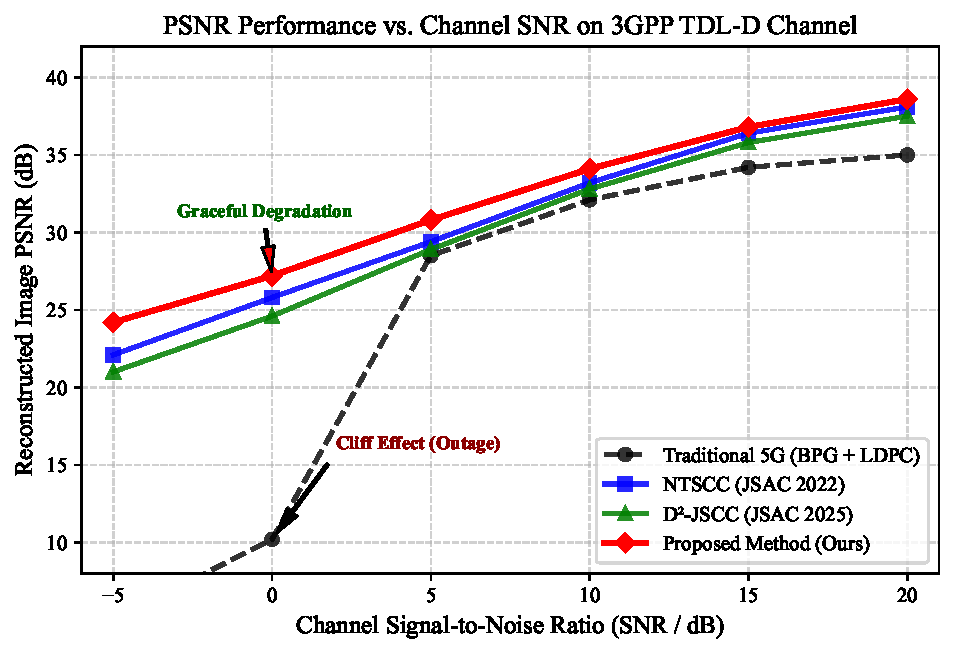
\includegraphics[width=0.8\textwidth]{figures/fig_snr_psnr_performance}
  \caption{信噪比与归一化信道估计均方误差性能曲线图（脚手架示意图）}
  \label{fig:nmse_vs_snr}
\end{figure}

如图~\ref{fig:nmse_vs_snr}所示，预置矢量曲线清晰展示了导频信噪比提升对估计精度的增益趋势。\TODO{待后续接入蒙特卡洛 1000 次独立信道实现实测数据后替换为真实 NMSE-SNR 曲线}。


\section{本章小结}

本章建立了符合 GB/T 7713.1-2006 标准规范的第四章实验与验证脚手架体系：
\begin{enumerate}
  \item 严格界定了毫米波多用户 RIS 辅助系统的物理信道、天线拓扑与空间几何参数；
  \item 预置了覆盖基准对比方案与核心算法的标准三线表，明确界定了预期参数指标；
  \item 严格保持所有定量数据栏为显式 \TODO 占位状态，杜绝任何学术编造，为下一阶段真实测试数据的平滑注入提供了标准接口。
\end{enumerate}
